\chapter{Sistema de telecomunicaciones}\label{comunicacion}
Se determinó utilizar la plataforma Arduino por su simplicidad en prototipado y programación, además de ser de fácil acceso y una tecnología escalable.
\section{ATMega328p}
Utilizando una placa Arduino Uno se comienza el prototipo del dispositivo que va a cumplir la función de tomar los datos de los sensores análogos. La versión de Arduino Uno utiliza un microcontrolador ATMega328 que posee 32[KB] de memoria de programa y una memoria RAM de 2[Mb]. Este consta de 1 puerto de comunicación UART y posee 32 pines de los cuales 23 pines son programables para entrada/salida como se muestra en la figura \ref{328}

\begin{figure}[H]
\centering
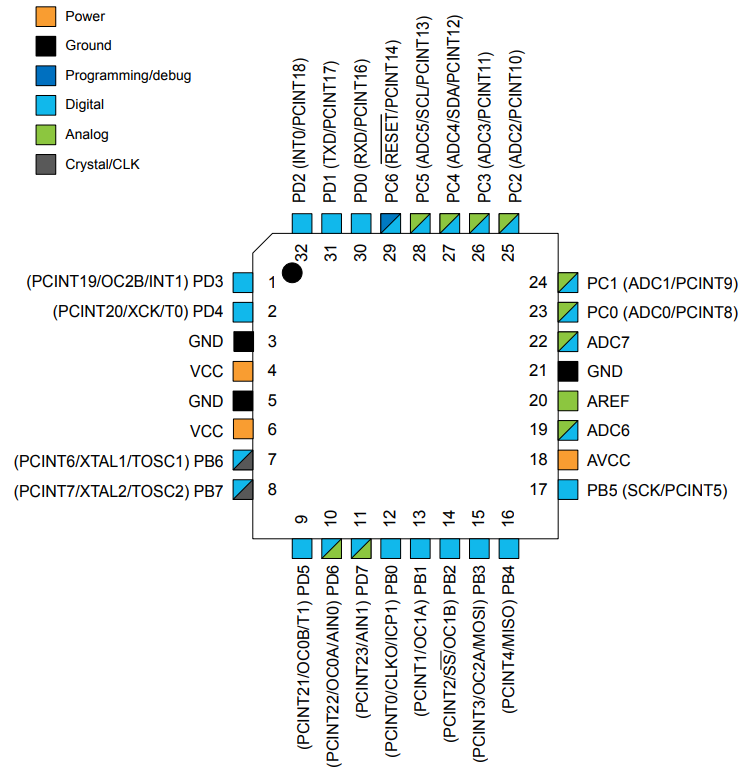
\includegraphics[scale=0.35]{figuras/mcu/328.png}
\caption{Microcontrolador ATMega328p}
\label{328}
\end{figure}

\section{ATMega2560}
Contrastando el modelo mostrado anteriormente, la placa Arduino Mega posee un microcontrolador ATMega2560 el cual incluye un aumento en todas sus capacidades. Comenzando con la capacidad de su memoria de programa, que asciende a 250[KB] y una memoria RAM de 8[KB]. Este microcontrolador posee 100 pines lo que incluye un aumento a 4 puertos de comunicación UART, además de aumento de entradas análogas y digitales. 

\begin{figure}[H]
\centering
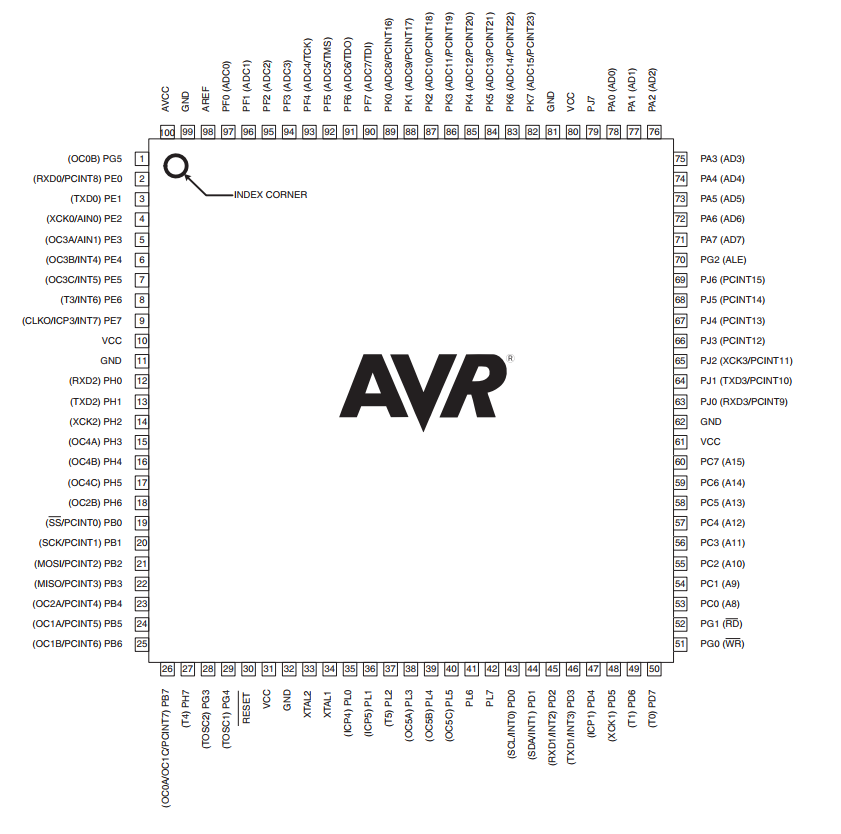
\includegraphics[scale=0.5]{figuras/mcu/2560.png}
\caption{Microcontrolador ATMega2560}
\label{mega}
\end{figure}

Como se puede observar en la figura \ref{mega}, hay un aumento considerable en las prestaciones que ofrece este microcontrolador con respecto al ATMega328p además de su tamaño. \\

Se va a trabajar en el diseño con este microcontrolador ya que posee 4 interfaces UART de las cuales una de estas siempre está definida para ser utilizada por la programación FTDl, esto se explicará mas adelante.\\

Esto involucra utilizar un chip con mayores capacidades de las necesarias pero esto es debido a la limitante de los microcontroladores utilizados por Arduino como se puede observar en la figura \ref{compara}.

\begin{figure}[H]
\centering
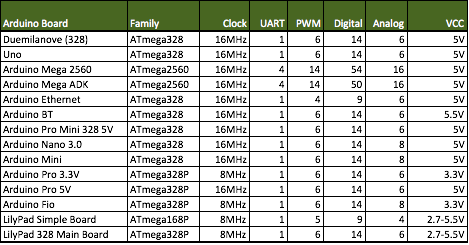
\includegraphics[scale=0.7]{figuras/mcu/compara.png}
\caption{Comparación microcontroladores Arduino}
\label{compara}
\end{figure}

Idealmente para el diseño del dispositivo, se utilizará un microcontrolador con 2 puertos UART ya que uno de estos es necesario para la comunicación con el computador y el otro es utilizado para el envío de información mediante bluetooth, pero por necesidad de rapidez para el diseño de prototipo y pruebas de sensores es necesario iterar con una placa ya fabricada para usos generales y disponibles en el mercado. Esto causaría una disminución significativa entre el precio del diseño del producto final. 
\newpage
\section{ATMega644PA}
Considerando la variable de costos es importante destacar una tercera opción para el diseño del dispositivo final. El microcontrolador ATMega644PA posee un menor conteo de pines ya que consta de 44 lo cual disminuye costos y tamaño a la hora del diseño. Con una memoria Flash de 64[KB] y memoria RAM de 4[KB]. Este provee 2 UART para la comunicación y los pines suficientes para sensores como se muestra en la figura \ref{644}.

\begin{figure}[H]
\centering
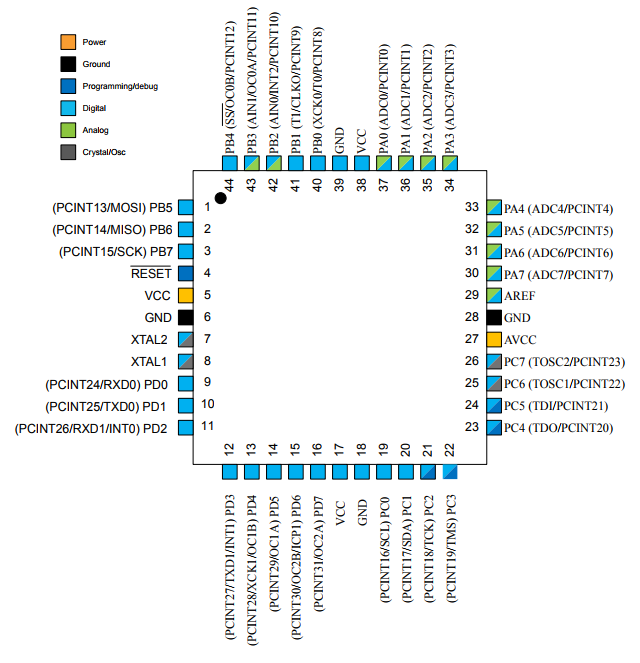
\includegraphics[scale=0.7]{figuras/mcu/644.png}
\caption{Microcontrolador ATMega644PA}
\label{644}
\end{figure}

Se puede observar en la imagen la disponibilidad de los puertos UART donde el Pin 9 y Pin 10 corresponden a UART0 considerado para la programación USB. Pin 11 y Pin 12 corresponden a UART1 que será utilizado para la comunicación con el dispositivo bluetooth.\\
En primera instancia se va a diseñar el dispositivo con el microcontrolador ATMega2560, debido a que existen modelos Arduino con esta misma componente y cumple los requisitos funcionales de poseer mas de 1 puerto UART. No es la opción ideal ya que posee mas prestaciones de las que se necesitan pero permite que se pueda prototipar inmediatamente  utilizando un Arduino equivalente, lo cual no se puede hacer con la versión ATMega644PA.

\section{Conclusiones}
Finalmente considerando las 3 opciones elegidas, se puede establecer una decisión final con respecto a cual microcontrolador utilizar.


\begin{table}[H]
\centering
\begin{tabular}{| c | c | c |}
\hline
\multicolumn{1}{|c|}{\textbf{Microcontrolador}}&
\multicolumn{1}{c|}{\textbf{Pines}}&
\multicolumn{1}{|c|}{\textbf{Precio (USD)}}\\ \hline
ATMega328p  & 32  & \$2.18  \\ \hline
ATMega2560  & 100 & \$12.44 \\ \hline
ATMega644PA & 44  & \$5.24  \\ \hline
\end{tabular}
\caption{Comparación microcontroladores}
\label{tablacompara}
\end{table}

Como se puede observar en la Tabla 1 se tomaron en cuenta los aspectos de tamaño y costos. ATMega328p se considera porque a pesar de que posee un solo puerto UART es posible utilizar otros pines para configurar comunicación serial por software (en comparación con la comunicación por hardware es mucho más lenta) lo cual será muy útil a la hora de hacer pruebas en toma de datos y envío de la información. En cuanto a precio y tamaño es una alternativa ideal ya que minimiza ambos aspectos. \\
La segunda opción siendo la que ofrece más opciones para sensores y memoria programable es excesivo para lo que se necesita desarrollar, pero se acerca más a los requerimientos necesarios que carece el microcontrolador ATMega328p. Esta opción tiene un el precio más elevado de las 3 opciones y por una diferencia considerable, es por esto que se utilizará para la primera versión del diseño final enfocado a tener un mínimo producto viable que funcione de la misma manera que el prototipo.\\
Finalmente la tercera opción siendo la más viable ya que posee un tamaño mucho menor al ATMega2560 y un precio menor a la mitad que este, ofrece todas las capacidades necesarias pero como se muestra en la figura \ref{compara}, no hay en el mercado una placa Arduino con este microcontrolador ni tampoco otra opción que cumpla con el requisito de utilizar 2 UART es por esto que como segunda iteración del producto final se debe buscar un bootloader compatible con el entorno de desarrollo Arduino para el ATMega644PA o trabajar en otra plataforma compatible con ese microcontrolador.


